%class
	\documentclass{beamer}

%template
	\usetheme{HannoverSalman}
	\setbeamertemplate{navigation symbols}{}
	%\setbeamertemplate{footline}{\centering{\insertframenumber/\insertpresentationendpage}}
	%\setbeamertemplate{footline}{\hspace*{.5cm}\scriptsize{\hfill\insertframenumber\hspace*{.5cm}}} 


%packages
	\usepackage{amsmath, amssymb, graphicx,cancel}
	\usepackage[absolute,overlay]{textpos}
	\usepackage{subfigure}
	\usepackage{caption}\captionsetup{labelformat=empty,labelsep=none}
	\usepackage{geometry}
	\geometry{verbose}
	\usepackage{color}
	\usepackage{xmpmulti}
	\usepackage[3D]{movie15}
	\usepackage{hyperref}
%	\usepackage{bookmark}
	\usepackage[open,openlevel=4,atend]{bookmark}
	%\bookmarksetup{color=blue}
	\usepackage{multirow}
	\usepackage[style=numeric,defernumbers, authoryear]{biblatex}
	%\usepackage[square,sort]{natbib}
	%\usepackage{fancyhdr}%\pagestyle{fancy} 

	
	\hypersetup{bookmarksdepth = 4}


%citations files
	\bibliography{MyCitations}

%logoCSIPCPL
    \setlength{\TPHorizModule}{1mm}
    \setlength{\TPVertModule}{1mm}
    \newcommand{\logoCSIPCPL}
    {
    	\begin{textblock}{1}(100,2) %(100,85)  for bottom
    		
\includegraphics[width=1.5cm]{figs/logo_CSIP}
    	\end{textblock}
    	
	\begin{textblock}{1}(117,1) %(117,85)  for bottom
    		
\includegraphics[width=1.0cm]{figs/logo_CPL}
    	\end{textblock} 
    }

%logo evolution
    \newcommand{\logoEvolution}
    {    	
	\begin{textblock}{1}(110,1) %(117,85)  for bottom
    		\includegraphics[width=0.65in]{figs/logo_evolution.pdf}
    	\end{textblock} 
    }

%logo Qualcomm
    \newcommand{\logoQualcomm}
    {
    	\begin{textblock}{1}(110,2) %(100,85)  for bottom
    		\includegraphics[width=1.5cm]{figs/logo_qualcomm.jpg}
    	\end{textblock}
    }
%logo Qualcomm (long)
    \newcommand{\logoQualcommllong}
    {
    	\begin{textblock}{1}(0,0) 
    		\includegraphics[width=1.25in]{figs/logo_qualcomm_long.jpg}
    	\end{textblock}
    }

%logo Tech Tower
    \newcommand{\logoTechTower}
    {
    	\begin{textblock}{1}(0,0) 
    		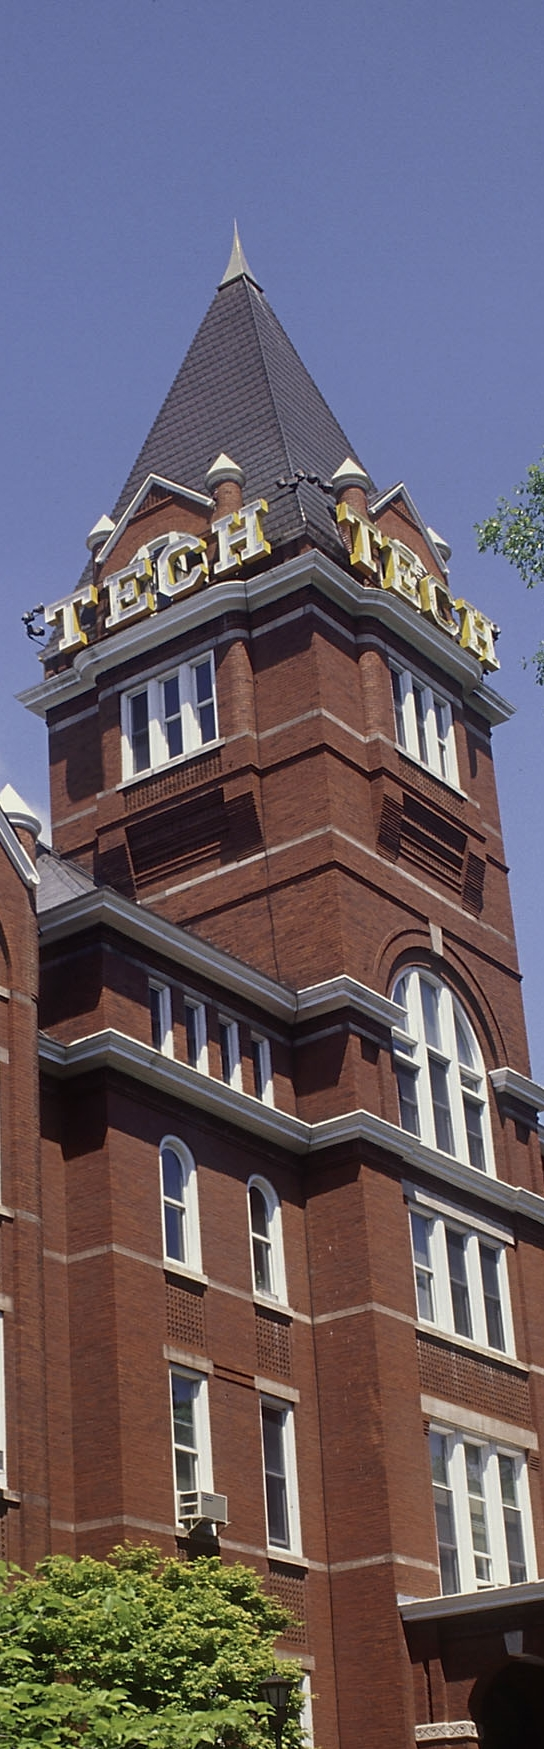
\includegraphics[width=1.25in]{figs/logo_TechTower.jpg}
    	\end{textblock}
    }

%logo tree
    \newcommand{\logoTree}
    {
    	\begin{textblock}{1}(0,0) 
    		\includegraphics[width=1.25in]{figs/logo_tree.jpg}
    	\end{textblock}
    }
%page numbers
    \newcommand{\mypagenum}
    {
    	\begin{textblock}{1}(1,94) 
		{\tiny \color[rgb]{0.2,0.2,1}\insertframenumber} %\insertframenumber,\insertpresentationendpage, \inserttotalframenumber
    	\end{textblock}
    }
%my footnote citation
	\newcommand{\myFootnoteCitation}[2]
	{
		\footnote{\tiny \citeauthor{#1}, \emph{#2}, \citeyear{#1}.}  %\citeauthor{#1}, \citetitle{#1}, #2 \citeyear{#1}.
	}
%my refer to citation
	\newcommand{\mycite}[1]
	{
		\emph{\citeauthor{#1} (\citeyear{#1})}
	}
%my footnote website citation
	\newcommand{\myFootnoteWebsiteCitation}[1]
	{
		\footnote{\tiny \citeauthor{#1}}
	}

\let\thefootnote\relax\footnotetext{Footnotetext without footnote mark}


%section underline
%\newcommand{\tmpsection}[1]{}
%\let\tmpsection=\section
%\renewcommand{\section}[1]{\tmpsection{\underline{#1}}}



%commands
	\newcommand{\likelihood}{p(Z_k| x_k) }						%likelihood
	\newcommand{\prior}{p(x_k)  } 								%prior
	\newcommand{\posterior} {p(x_k| Z_k)}						%posterior
	\newcommand{\prediction} {p(x_k| Z_{k-1})}					%prediction
	\newcommand{\update} {p(x_k|Z_k)}							%update
	\newcommand{\observations} {p(Z_k)}						%observations
	\newcommand{\prevobservations} {p(Z_{k-1})}				%previous observations
	\newcommand{\dxpk} {dx_{k-1}}							%dx_{k-1}
	\newcommand{\ChapKolm}{\int{p(x_k| x_{k-1})p(x_{k-1}|Z_{k-1})} \dxpk} %Chapman Kolmogorov

	%algorithm specific: JPDAF
	\newcommand{\likelihoodJPDAF}{p(Z_k| \chi, m, Z_{k-1}) }		%1. likelihood
	\newcommand{\priorJPDAF}{p(\chi|m, Z^{k-1}} 				%2. prior	
	\newcommand{\observationsJPDAF} {p(Z_k}					%3. observations
	\newcommand{\posteriorJPDAF} {p(\chi| Z_k)}					%4. posterior

%environments
	\newenvironment{changemargin}[2]
	{
	  	\begin{list}{}
		{
			\setlength{\topsep}{0pt}%
			\setlength{\leftmargin}{#1}%
			\setlength{\rightmargin}{#2}%
			\setlength{\listparindent}{\parindent}%
			\setlength{\itemindent}{\parindent}%
			\setlength{\parsep}{\parskip}%
		}
	  	\item[]
		}
		{\end{list}
	}
%figures

%colors
\definecolor{darkgreen}{rgb}{0,0.5,0}

%personal details
	\author{Salman Aslam}
	\institute{Advisor, Dr Christopher Barnes (ECE)\\Co-advisor, Dr Aaron Bobick (CoC)\\Georgia Institute of Technology}
	\date{}

\begin{document}
%####################################################################################################
\title{Robust, Real-time \\Vehicle Contour Tracking \\on \\Low Quality Aerial Infra Red Imagery}
%####################################################################################################


\begin{frame}[plain]
\logoTechTower\logoCSIPCPL
	\titlepage
\end{frame}


\begin{frame}
\frametitle{Outline}
\logoTechTower\logoCSIPCPL
	\tableofcontents
\end{frame}



%####################################################################################################
\section{Introduction}
%####################################################################################################
\begin{frame}
\frametitle{Introduction}
\logoCSIPCPL\mypagenum
	\begin{itemize}
		\item {\color{red} Imagery:} 
			\begin{itemize}
				\item Infra-red
				\item low contrast, gray-scale
			\end{itemize}
		\item {\color{red} Camera:} 
			\begin{itemize}
				\item aerial, moving (hovering over target)
				\item no background or target motion model
			\end{itemize}
		\item  {\color{red} Prior information:} 
			\begin{itemize}
				\item In IR images, corners can be strong in vicinity of vehicle contour
			\end{itemize}
	\end{itemize}
\end{frame}

%====================
\subsection{Scenario}
%====================

\begin{frame}
\frametitle{Tracking scenario}
\logoCSIPCPL\mypagenum	
		\multiinclude[<+>][format=jpg, start=0, graphics={width=0.8\textwidth}]{figs/TRK_IGARSS2010_contour_scenario}
\end{frame}




%			\begin{itemize}
%				\item Computationally expensive
%				\item Dependent on good initialization
%			\end{itemize}


%====================
\subsection{Contour representation}
%====================

\begin{frame}
\frametitle{Contour representation}
\framesubtitle{Polynomials}
\logoCSIPCPL\mypagenum
	\begin{figure}
		\includegraphics[width=1.0\textwidth]{figs/theory_contour_PolynomialFitting.pdf}
	\end{figure}
\end{frame}


\begin{frame}
\frametitle{Contour representation}
\framesubtitle{Elliptical Fourier components}
\logoCSIPCPL\mypagenum
	\begin{figure}
		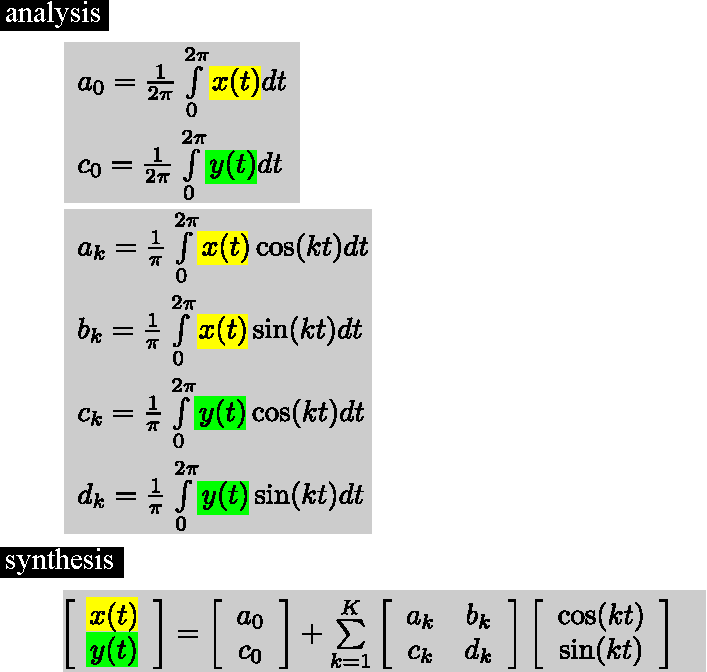
\includegraphics[height=0.8\textheight]{figs/theory_curves_ellipticalFourier.pdf}
	\end{figure}
\end{frame}


\begin{frame}[plain]
\frametitle{Contour representation}
\framesubtitle{splines}
	\begin{changemargin}{-1.3in}{0in} 
		\begin{figure}
			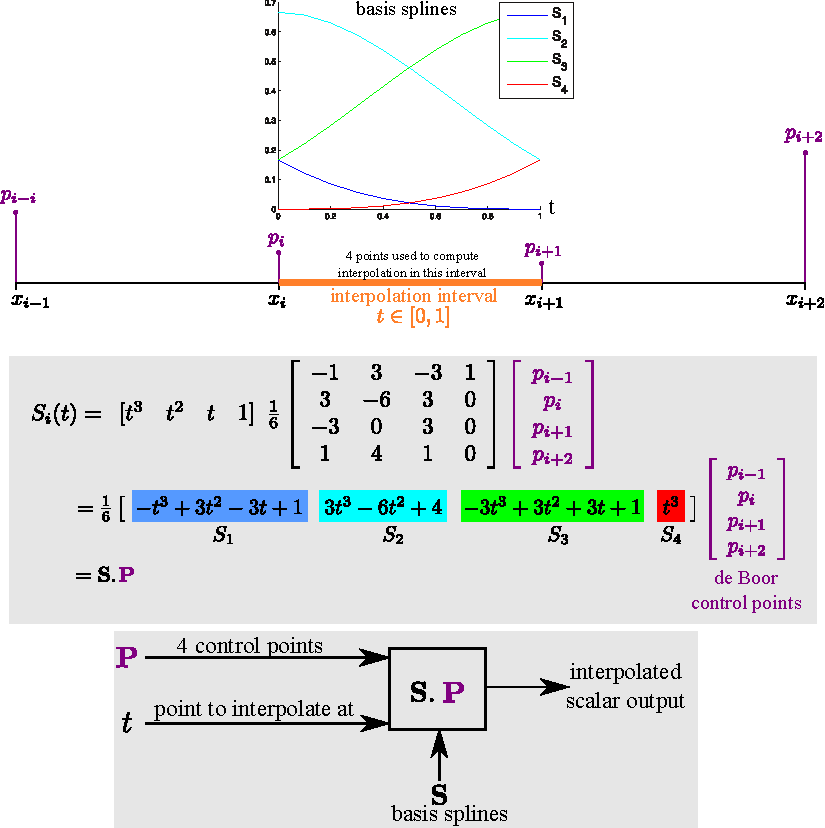
\includegraphics[height=0.85\textheight]{figs/theory_curves_UniformCubicBsplines.pdf}
		\end{figure}
	\end{changemargin}
\end{frame}



%====================
\subsection{Contour evolution}
%====================
\begin{frame}
\frametitle{Contour evolution}
\framesubtitle{snakes}
\logoCSIPCPL\mypagenum
	\begin{figure}
		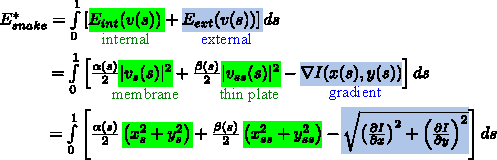
\includegraphics[width=1.0\textwidth]{figs/theory_curves_snakes.pdf}
	\end{figure}
\end{frame}

\begin{frame}
\frametitle{Contour evolution}
\framesubtitle{energy minimization}
\logoCSIPCPL\mypagenum
	%\begin{itemize}
	%	\item Even though the curve has corners, the first derivative remains small
	%\end{itemize}
	\begin{figure}
		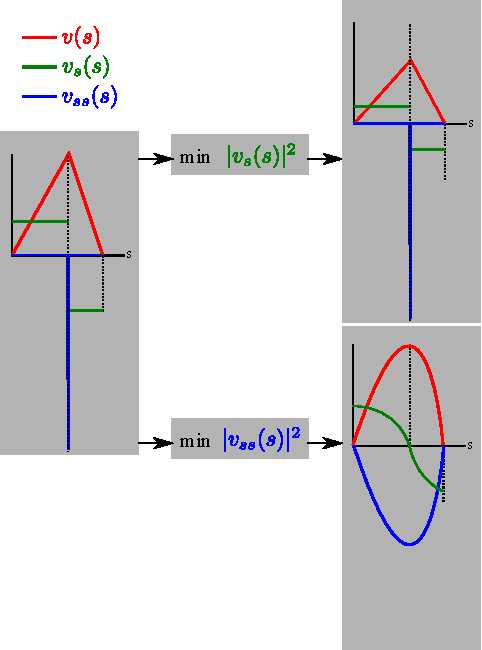
\includegraphics[height=0.8\textheight]{figs/TRK_contours.pdf}
	\end{figure}
\end{frame}



\begin{frame}
\frametitle{Contour evolution}
\framesubtitle{Elliptical Fourier + snakes}
\logoCSIPCPL\mypagenum
	\begin{figure}
		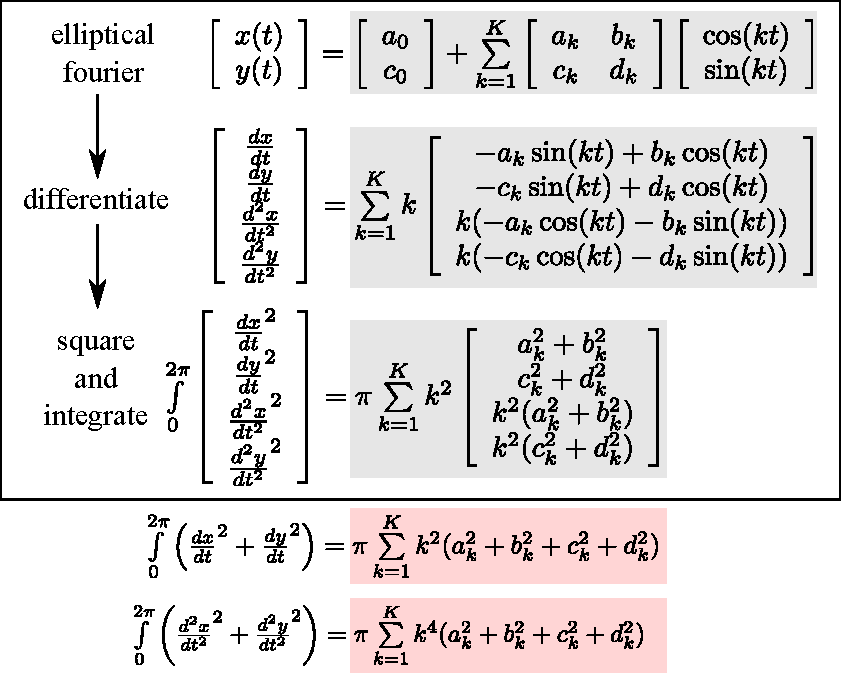
\includegraphics[width=0.9\textwidth]{figs/theory_curves_ellipticalFourierSnakes.pdf}
	\end{figure}
\end{frame}


%====================
\subsection{Contour tracking}
%====================
\begin{frame}
\frametitle{Contour tracking}
\framesubtitle{introduction}
\logoCSIPCPL\mypagenum
	\begin{enumerate}
		\item Parameterize curve to get shape parameter $\mathbf{x}$
			\begin{itemize}
				\item example, use B-spline curves
				\item control points could be used, but this would allow too many degrees of freedom
				\item create shape space
			\end{itemize}
		\item Predict: Markov-chain model in shape space
		\item Update: Fuse information from prediction and observation
			\begin{itemize}
				\item Kalman filter
				\item Particle filter
			\end{itemize}
	\end{enumerate}
\end{frame}

\begin{frame}
\frametitle{Contour tracking}
\framesubtitle{big picture}
\logoCSIPCPL\mypagenum
	\begin{figure}
		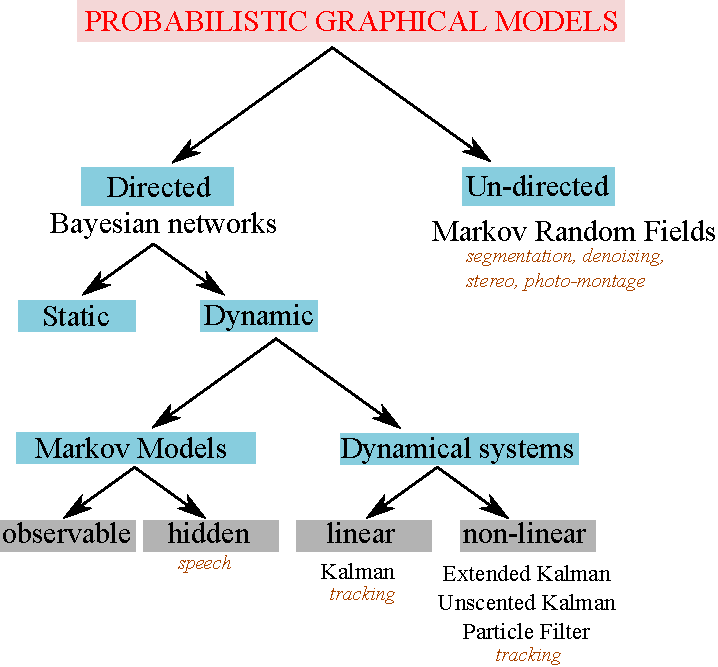
\includegraphics[width=0.9\textwidth]{figs/PRML_PGM_overview.pdf}
	\end{figure}
\end{frame}


\begin{frame}
\frametitle{Contour tracking}
\framesubtitle{Kalman filter}
\logoCSIPCPL\mypagenum
	\begin{figure}
		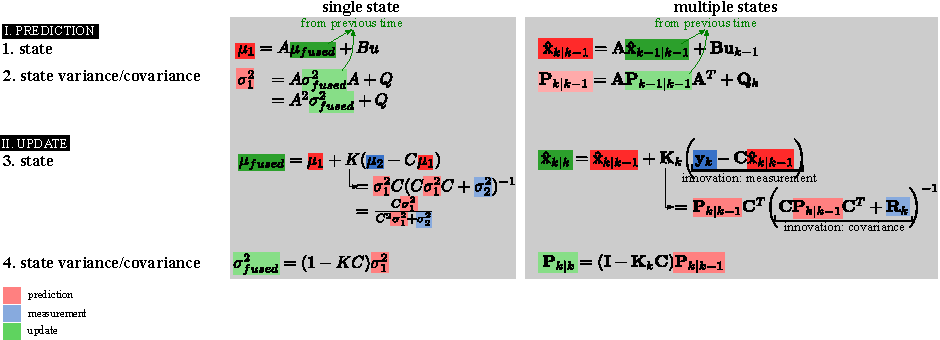
\includegraphics[width=1.0\textwidth]{figs/TRK_KalmanFilter_equations.pdf}
	\end{figure}
\end{frame}


\begin{frame}
\frametitle{Contour tracking}
\framesubtitle{Particle Filter}
\logoCSIPCPL\mypagenum
	\begin{figure}
		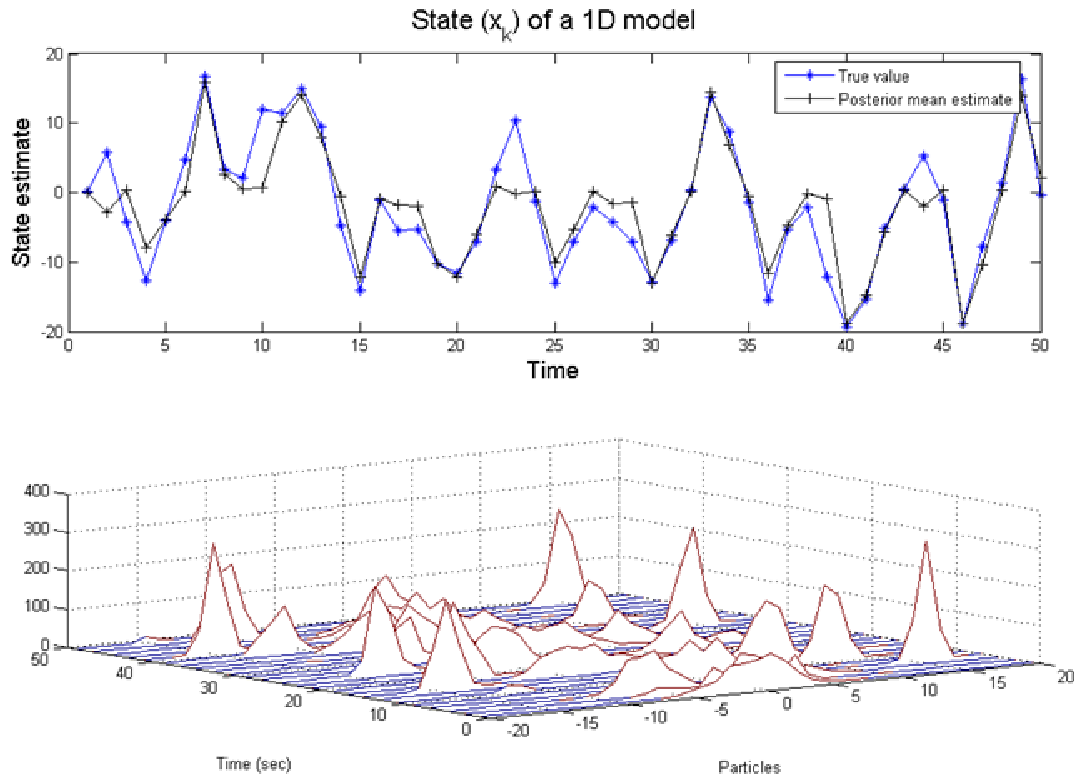
\includegraphics[width=1.0\textwidth]{figs/TRK_ParticleFilter_multimodalPDF.pdf}
		\caption{Multi-modal PDF}
	\end{figure}	
\end{frame}



%####################################################################################################
\section{Experiments}
%####################################################################################################
\begin{frame}
\frametitle{Experiments}
\framesubtitle{our approach}
\logoCSIPCPL\mypagenum
	{\color{red}Commonly used method}: Using a Markov-chain model in shape space for prediction and fusion (can be expensive)
	
	{\color{red}Our approach}:
	\begin{itemize}
		\item Use a simple method to get estimate of target contour
		\item May be enough for certain applications
		\item Drawing contours using Fourier descriptors
			\begin{itemize}
				\item computationally efficient
				\item Vehicle contour in overhead imagery can be approximated with few elliptical Fourier components
			\end{itemize}
		\item Occasional localization/correction using energy minimization (snakes) with Fourier descriptors is also computationally efficient
	\end{itemize}
\end{frame}




\begin{frame}
\frametitle{Experiments}
\framesubtitle{steps}
\logoCSIPCPL\mypagenum
		\begin{enumerate}
		\item {\color{red}Target initialization}
			\begin{itemize}
				\item 4 or more corners selected on contour
			\end{itemize}
		\item {\color{red}Inter-frame matching}
			\begin{itemize}
				\item corners matched in subsequent frames
			\end{itemize}
		\item {\color{red}Contour generation}
			\begin{itemize}
				\item elliptical Fourier contours drawn using corners as anchor points 
				\item rotation invariance
			\end{itemize}
		\item {\color{red}drift avoidance}
			\begin{itemize}
				\item occasional correction incorporating energy minimization (snakes)
			\end{itemize}
	\end{enumerate}
\end{frame}



%####################################################################################################
\section{Results}
%####################################################################################################
\begin{frame}[plain]
\frametitle{Results}
\framesubtitle{Elliptical Fourier descriptors}
\mypagenum
	\begin{changemargin}{-1.3in}{0in}
		\multiinclude[<+>][format=png, start=0, graphics={width=1.35\textwidth}]{figs/TRK_IGARSS2010_contour_ellipFourier}
	\end{changemargin}
\end{frame}





\begin{frame}
\frametitle{Results}
\framesubtitle{Elliptical Fourier descriptors}
\logoCSIPCPL\mypagenum
	Corners can be inside contour, causing it to shrink
	\begin{columns}
		\begin{column}{1in}

			\begin{figure}
				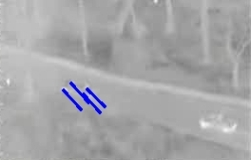
\includegraphics[width=1.5\textwidth]{figs/TRK_IGARSS2010_matching_0_30.jpg}
			\end{figure}
			\begin{figure}
				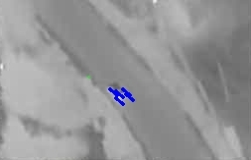
\includegraphics[width=1.5\textwidth]{figs/TRK_IGARSS2010_matching_1250_1277.jpg}
			\end{figure}
		\end{column}
		\begin{column}{1in}
			\begin{figure}
				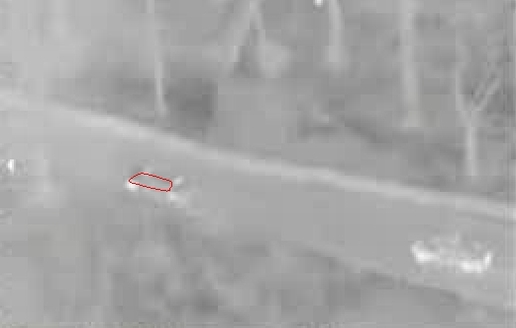
\includegraphics[width=1.5\textwidth]{figs/TRK_IGARSS2010_00030_contour.jpg}
			\end{figure}
			\begin{figure}
				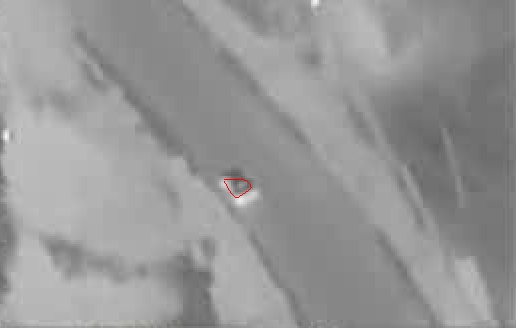
\includegraphics[width=1.5\textwidth]{figs/TRK_IGARSS2010_01277_contour.jpg}
			\end{figure}
		\end{column}			
	\end{columns}
\end{frame}




\begin{frame}
\frametitle{Results}
\framesubtitle{Localization with Snakes \\{\small(with Elliptical Fourier representation)}}
\logoCSIPCPL\mypagenum
		\multiinclude[<+>][format=jpg, start=0, graphics={width=1.0\textwidth}]{figs/TRK_IGARSS2010_FN_00000_snakes}
\end{frame}



\begin{frame}[plain]
\frametitle{Results}
\framesubtitle{Elliptical Fourier descriptors}
\mypagenum
	\begin{changemargin}{-1.3in}{0in}
		\multiinclude[<+>][format=png, start=0, graphics={width=1.35\textwidth}]{figs/TRK_IGARSS2010_contour_ellipFourier}
	\end{changemargin}
\end{frame}





\begin{frame}
\frametitle{Results}
\framesubtitle{Elliptical Fourier descriptors}
\logoCSIPCPL\mypagenum
	Corners can be inside contour, causing it to shrink
	\begin{columns}
		\begin{column}{1in}

			\begin{figure}
				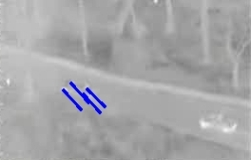
\includegraphics[width=1.5\textwidth]{figs/TRK_IGARSS2010_matching_0_30.jpg}
			\end{figure}
			\begin{figure}
				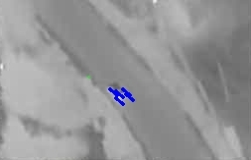
\includegraphics[width=1.5\textwidth]{figs/TRK_IGARSS2010_matching_1250_1277.jpg}
			\end{figure}
		\end{column}
		\begin{column}{1in}
			\begin{figure}
				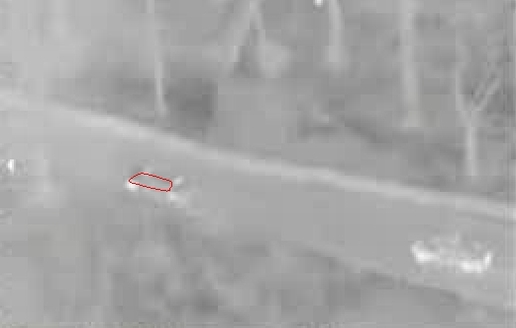
\includegraphics[width=1.5\textwidth]{figs/TRK_IGARSS2010_00030_contour.jpg}
			\end{figure}
			\begin{figure}
				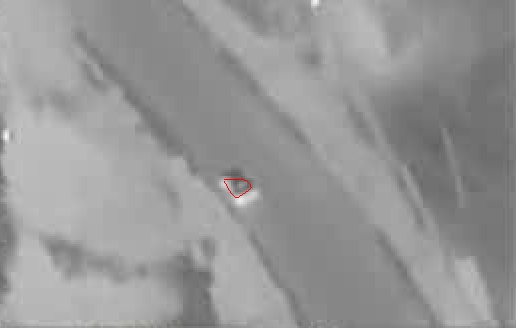
\includegraphics[width=1.5\textwidth]{figs/TRK_IGARSS2010_01277_contour.jpg}
			\end{figure}
		\end{column}			
	\end{columns}
\end{frame}




\begin{frame}
\frametitle{Results}
\framesubtitle{Localization with Snakes \\{\small(with Elliptical Fourier representation)}}
\logoCSIPCPL\mypagenum
		\multiinclude[<+>][format=jpg, start=0, graphics={width=1.0\textwidth}]{figs/TRK_IGARSS2010_FN_00000_snakes}
\end{frame}


%####################################################################################################
\section{Conclusions}
%####################################################################################################

\begin{frame}
\frametitle{Conclusions}
\logoCSIPCPL\mypagenum
	\begin{itemize}
		\item Elliptical fourier descriptor based contours are a "reasonable" estimate for vehicle contours in IR imagery
		\item This method can be used in conjunction with more computationally expensive methods
		\item However, in certain cases, contours can shrink to inside of contour
	\end{itemize}
\end{frame}





%####################################################################################################
%####################################################################################################
%\bibliographystyle{ieee}
%\bibliography{c:/salman/work/writing/MyCitations}
\end{document}
%####################################################################################################

%####################################################################################################

